\chapter{Transcriptional noise and exaptation as sources for bacterial sRNAs}


\section{Preface}
"2.	The significance of the supervisor’s contribution often justifies co-authorship of submitted or published work. An appropriate level of independence on the part of the student is expected. The examination rules specify that if parts of the thesis are based on published work under joint authorship, the supervisor should provide a statement about the extent to which this is the candidate’s own work."
\par
"Important Note: When including material from publications in a thesis, students should be aware of the copyright policies of journals. It is recommended that students request journals to vary their normal copyright agreements to allow material from an article to be included in a thesis (as the thesis will be publicly available through the University’s Library). For more information on copyright, please go to the University’s Thesis Information page.

"

Bethany R Jose \textsuperscript{1,2,*}, Paul P Gardner \textsuperscript{1,2}, Lars Barquist \textsuperscript{3,4,*} 

keywords: sRNAs, ncRNA, bacteria, selection, transcriptional noise, \textit{de novo} evolution, exaptation

\begin{enumerate}
    \item Biomolecular Interactions Centre, School of Biological Sciences, University of Canterbury, Christchurch, New Zealand.
    \item Department of Biochemistry, Otago University, Dunedin, New Zealand.
    \item Helmholtz Institute for RNA-based Infection Research (HIRI), Helmholtz-Centre for Infection Research (HZI), Würzburg, Germany.
    \item Faculty of Medicine, University of Würzburg, Würzburg, Germany. 
\end{enumerate}

\textsuperscript{*}Correspondence to: bethany.jose@postgrad.otago.ac.nz, lars.barquist@helmholtz-hiri.de
\section{Abstract}
Understanding how new genes originate and integrate into cellular networks is key to understanding evolution. Bacteria present unique opportunities for both the natural history and experimental study of gene origins, due to their large effective population sizes, rapid generation times, and ease of genetic manipulation. Bacterial small non-coding RNAs (sRNAs) in particular, many of which operate through a simple antisense regulatory logic, may serve as tractable models for exploring processes of gene origin and adaptation. Understanding how and on what timescales these regulatory molecules arise has important implications for understanding the evolution of bacterial regulatory networks, in particular for the design of comparative studies of sRNA function. Here we introduce relevant concepts from evolutionary biology and review recent work that has begun to shed light on the timescales and processes through which non-functional transcriptional noise is co-opted to provide regulatory functions. We explore possible scenarios for sRNA origin, focusing on the co-option, or exaptation, of existing genomic structures which may provide protected spaces for sRNA evolution.

\section{Introduction}

Far from being relics of a lost RNA world \citep{Eddy2001-jv}, most bacterial non-coding RNAs (ncRNAs) appear to be relatively recent innovations, with only a handful that are involved in translation, transcription, and translocation exhibiting deep conservation \citep{Hoeppner2012-pl} (Figure \ref{fig:conserved_rnas}).
One class of bacterial ncRNA that appears to be exceptionally dynamic over evolutionary time are the small non-coding RNAs (sRNAs) --- functionally heterogeneous transcripts of around 50--500 nucleotides, the majority of which appear to base-pair with mRNA targets to affect translation and/or mRNA stability \citep{Gorski2017-wu}.
Many of these functions are mediated by RNA-binding proteins, such as Hfq \citep{Vogel2011-gh}, though some operate by sequestering RNA-binding proteins, such as the global regulator CsrA \citep{Romeo2018-wb} or RNA polymerase \citep{Wassarman2007-de}.
\par

\begin{figure}[H]
  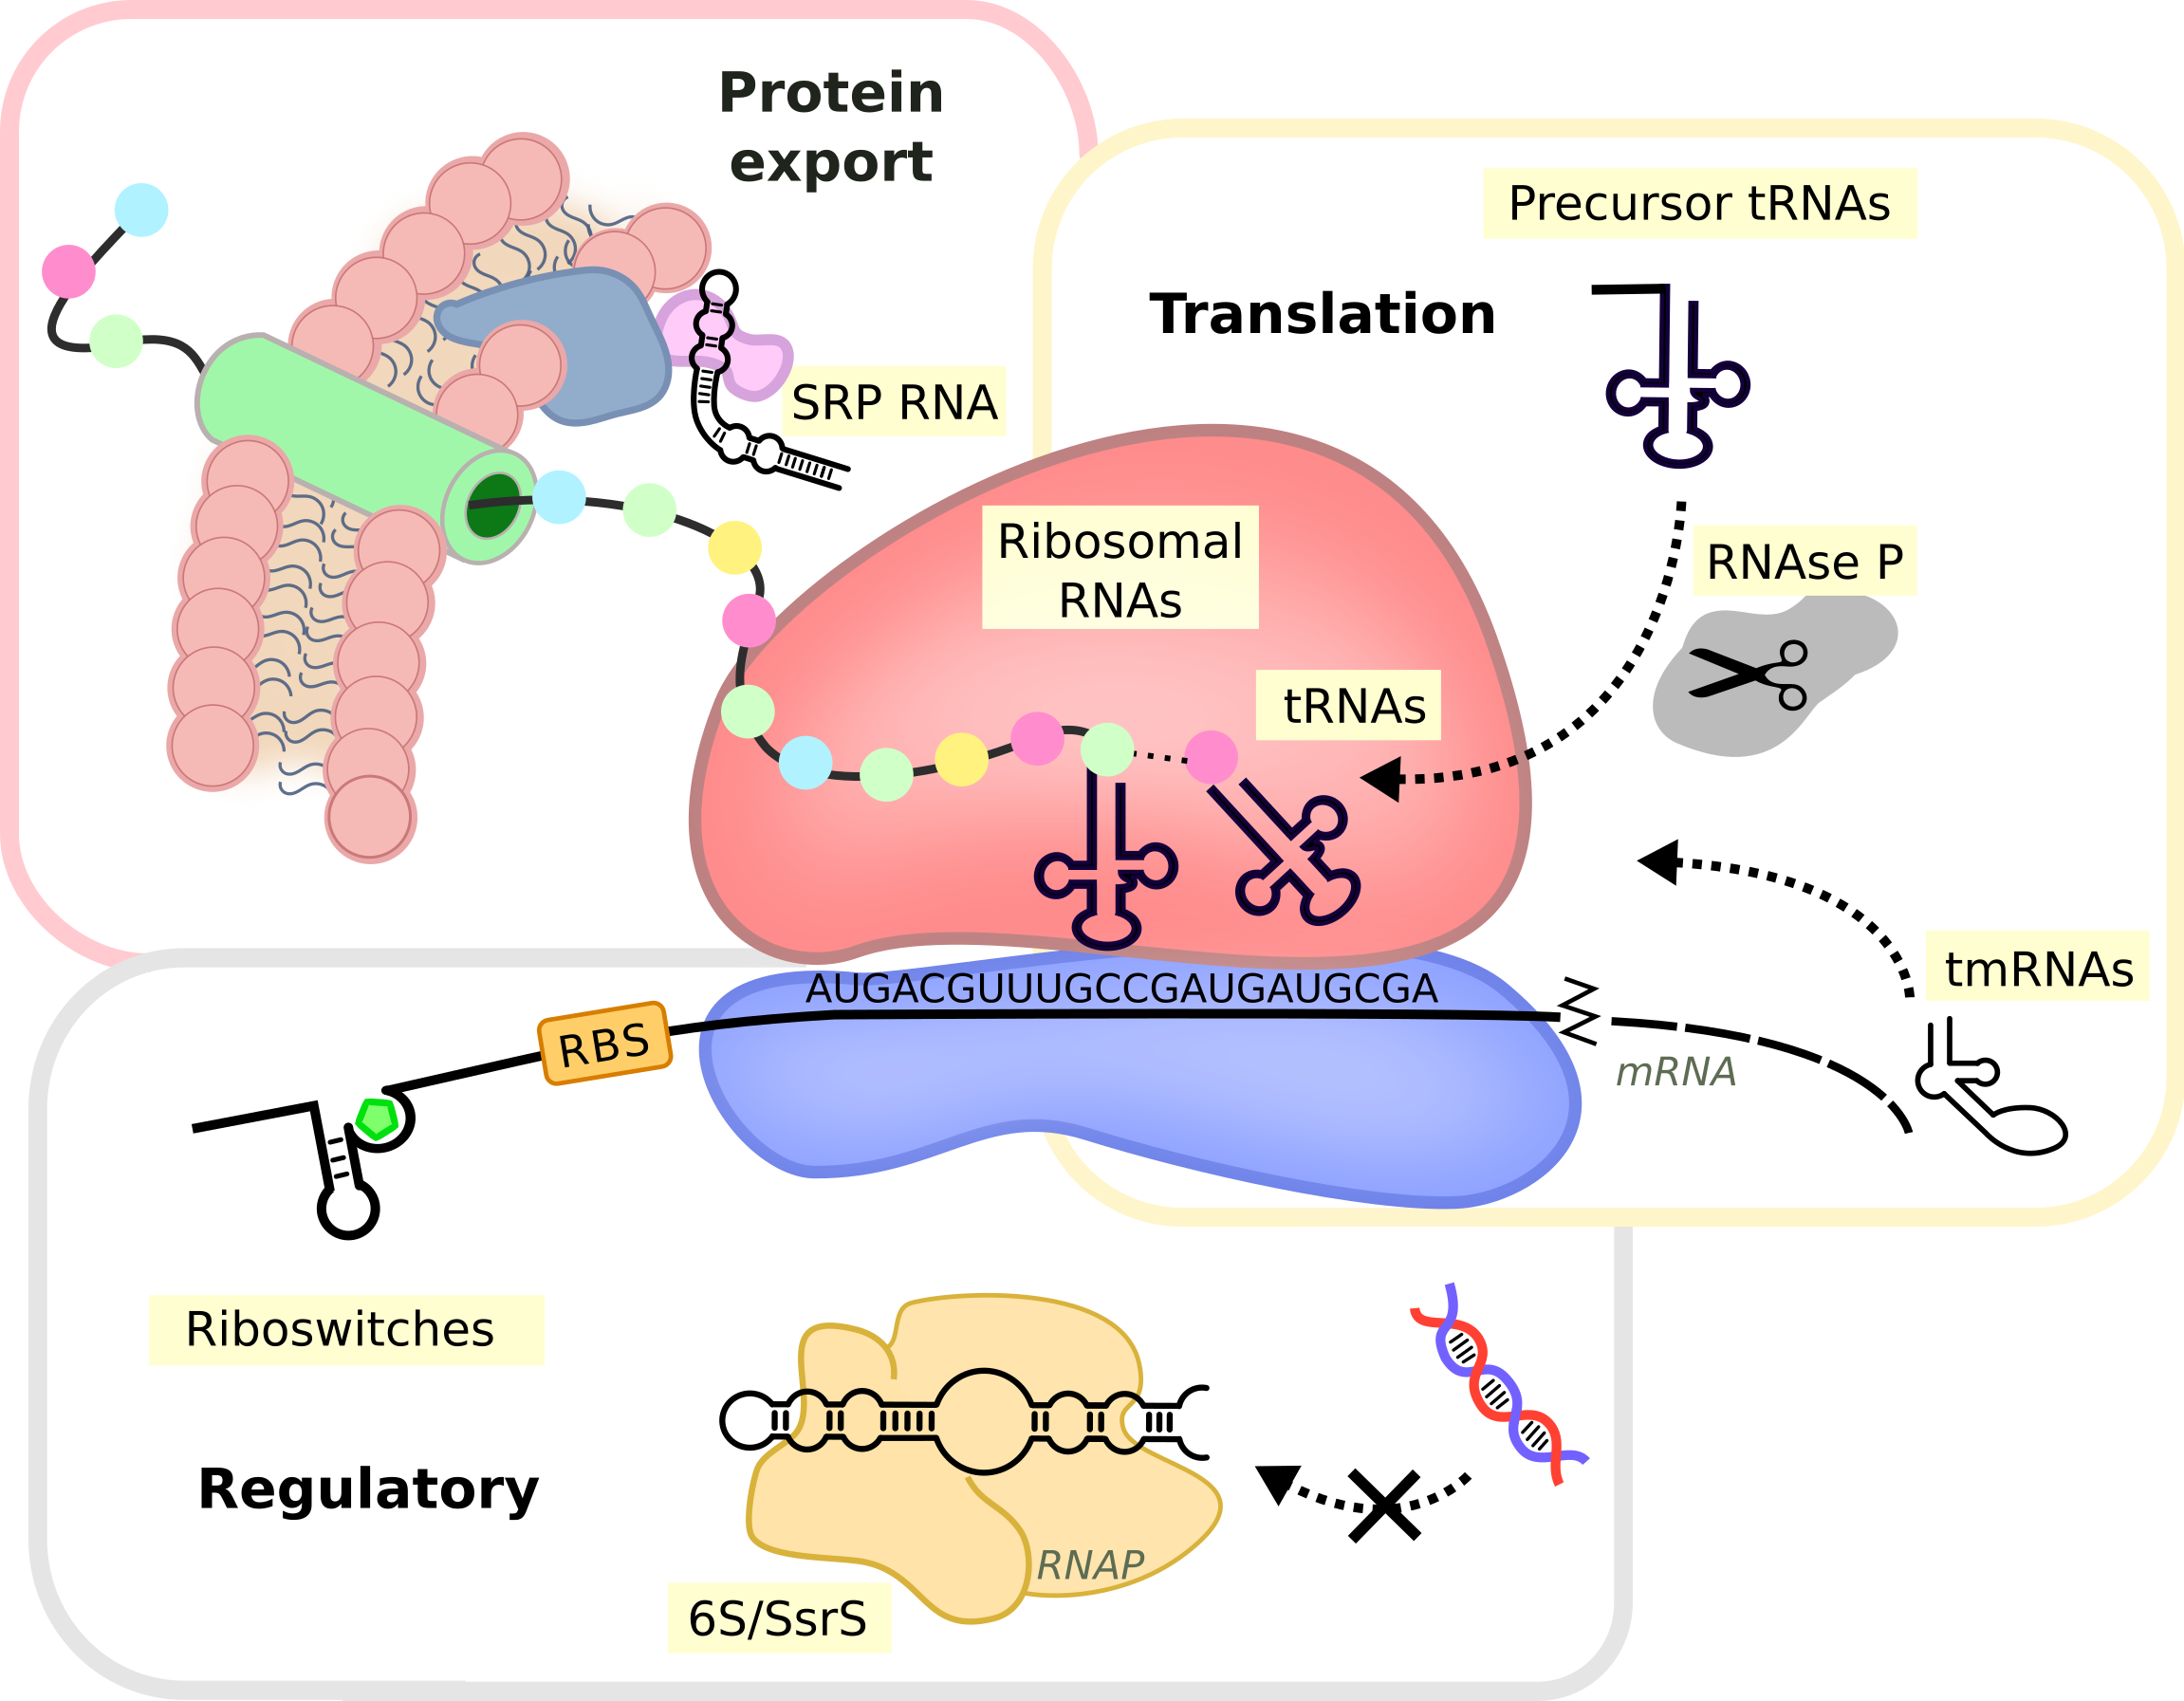
\includegraphics[scale=0.8]{lit_review/conserved_rnas_final_2.png}
  \caption{ Broadly conserved ncRNAs in bacteria. These ncRNAs are involved in core cellular processes: Translation (ribosomal RNAs, tRNAs, RNAse P, and tmRNAs), regulation of transcription (the 6S RNA, aka SsrS) and translation (TPP riboswitch, aka Thi-element), and protein export (the Signal Recognition Particle (SRP) RNA, aka 4.5S). Conserved ncRNAs were identified by phylogenetic distribution of ncRNA annotations in the Rfam database \citep{Hoeppner2012-pl}}
  \label{fig:conserved_rnas}
\end{figure}

The development of RNA-seq-based techniques to identify transcripts has led to an explosion of uncharacterised putative sRNAs \citep{Barquist2015-ta}, with whole-genome screens regularly reporting hundreds of novel sRNAs per genome \citep{Miotto2012-uw,Gomez-Lozano2015-yx,Kroger2012-jq,Rau2015-gt}. While functional roles for sRNAs are well established in the Proteobacteria \textit{Escherichia coli} and \textit{Salmonella enterica}, the continuing discovery of sRNAs in other phyla, such as \textit{Cyanobacteria} \citep{Klahn2015-pv} and \textit{Firmicutes} \citep{Durand2017-bc}, indicate that sRNA-based regulation is prevalent across the bacterial phylogeny. \par

While sRNAs appear to be a widespread feature of bacterial transcriptomes, individual sRNA loci themselves are generally not. BLAST-based analyses of \textit{Escherichia} \citep{Peer2014-yn}, \textit{Salmonella} \citep{Kroger2012-jq,Kroger2013-go}, \textit{Listeria} \citep{Cerutti2017-ip} and \textit{Campylobacter} \citep{Dugar2013-nt} sRNAs indicate that the majority are order or genus-specific, with some specific to serovars or even strains. It could be argued this result is an artifact of the sensitivity of homology search tools, as the lower bound for local alignment of nucleotide sequences is around \textasciitilde50-60\% sequence identity \citep{Gardner2005-la}, and sRNAs may be relatively robust to mutation given that their function is primarily attributed to "seed regions" of complementarity to their targets that may be as short as 6--8 nt\citep{Papenfort2010-ra, Richter2012-tt}. However, phylogeny-wide analysis of ncRNA conservation with more sensitive methods, including both profile hidden Markov models (HMMs) and curated covariance models (CMs) from the Rfam database \citep{Nawrocki2015-tt}, suggests a similar overall pattern of narrow conservation, with a sharp drop in the number of conserved ncRNAs at the genus to family level \citep{Lindgreen2014-dk} (Figure \ref{fig:lindgreen}). It is important to note that this analysis will overestimate conservation, since Rfam families are overwhelmingly constructed from conserved sequences. This lead us previously to propose a narrow "Goldilocks Zone" where comparative transcriptomics studies would be most useful for identifying conserved transcripts \citep{Lindgreen2014-dk}.

\begin{figure}[H]
  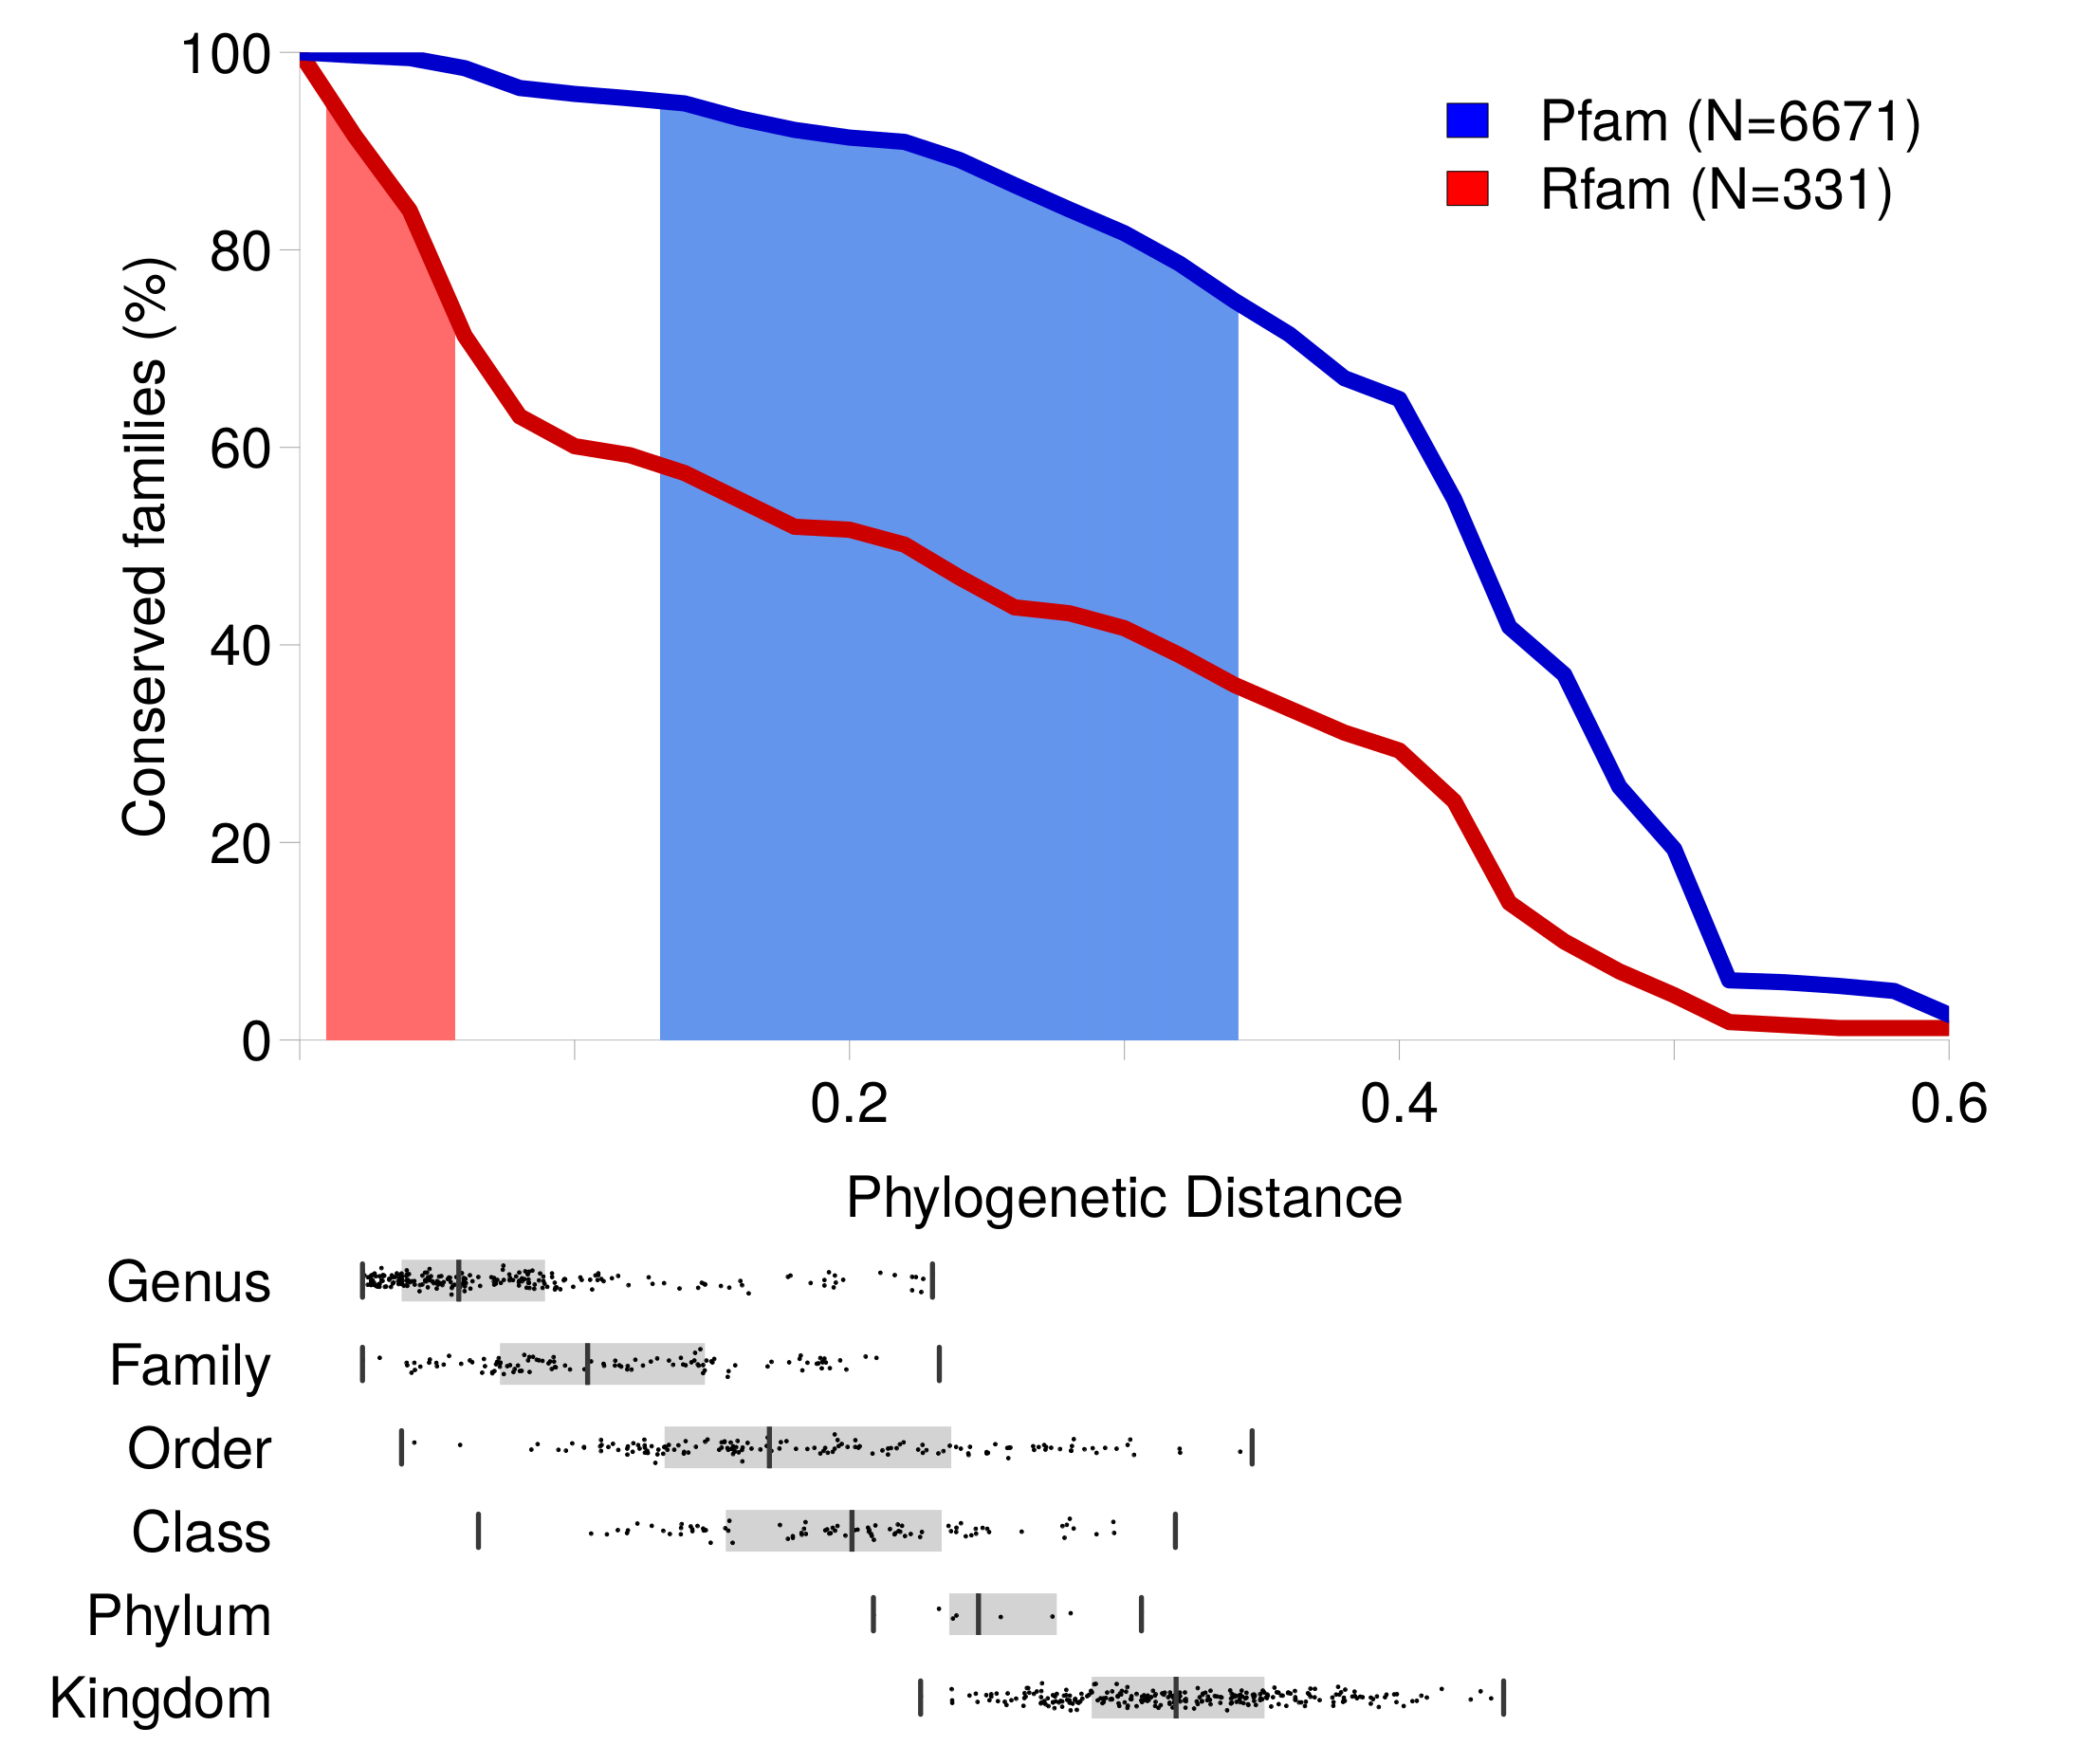
\includegraphics[scale=0.1]{lit_review/lindgreen.png}
  \caption{A comparison of conservation of RNA and protein families. Rfam and Pfam families were identified in 2,562 bacterial genomes using the Infernal and HMMER packages, respectively. The maximum phylogenetic distance spanned by each family was estimated using pairwise phylogenetic distances estimated from 16S rRNA sequences. Top: The percentage of Rfam (N=331) or Pfam (N=6,671) families that are conserved over phylogenetic distances ranging from 0 (closely related) to 0.6 (very divergent). The shaded regions under the curves indicate the “Goldilocks” phylogenetic ranges where between 95 and 75\% of RNA (light red) or protein (light blue) families are conserved. Bottom: The distribution of phylogenetic distances between randomly sampled pairs of genomes at 6 taxonomic ranks: genus, family, order, class, phylum and kingdom. At each taxonomic level, pairs were chosen from e.g. the same genus but different species, and so on up the taxonomic hierarchy until pairs of species from the same kingdom (bacteria) and different phyla are shown. Figure adapted from \citep{Lindgreen2014-dk}.}
  \label{fig:lindgreen}
\end{figure}
     
The near universal presence of a large cohort of non-coding transcripts paired with their apparent narrow conservation raises a number of questions: where do these transcripts come from? How are they turned over? How many serve biological functions in the cell, and how many are just transcriptional noise? Two excellent recent reviews have addressed how specific features of sRNA evolution may have evolved \citep{Updegrove2015-qr, Dutcher2018-ku}. Here we aim to complement this previous work by investigating evolutionary dynamics underlying the generation and removal of transcriptional noise, and how this could serve as the raw stuff from which functional sRNAs emerge.

\section{Transcriptional noise}

What do we mean by transcriptional noise? The term has been used to discuss ‘noisy’ interactions between the transcriptional machinery and DNA, in at least four distinct senses \citep{Raser2005-hm}. In this article, we use it in the sense of non-functional transcripts that accumulate over evolutionary time due the interaction of permissive transcriptional machinery with random mutations in the genome \citep{Struhl2007-ry} — however, it should be noted that even the concept of “function” is subject to multiple, competing definitions \citep{Doolittle2018-ha}.\par 

To clarify the sense in which we use the term transcriptional noise here, the Random Genome Project, a thought experiment proposed by Sean Eddy \citep{Eddy2013-fa}, is illustrative. Given the low information content of many protein binding sites, we would expect that any sufficiently long random DNA sequence will reproducibly interact with DNA-binding proteins, such as transcription factors. This will lead to the generation of discrete non-coding transcripts indistinguishable from native transcripts, including for instance condition-specific expression or affinity for RNA-binding proteins. By extension, random mutation will similarly lead to the generation of new, discrete transcripts over time as the accumulation of small changes lead to the generation of promoter-like sequences. Some proportion of these nascent transcripts will fix in the population depending on the effectiveness of selection and the dynamics of the host genome (Figure \ref{fig:transcriptional_noise}), discussed below. Importantly in the absence of perfectly efficient selection, a beneficial function is not a necessary condition for fixation.

\begin{figure}[H]
  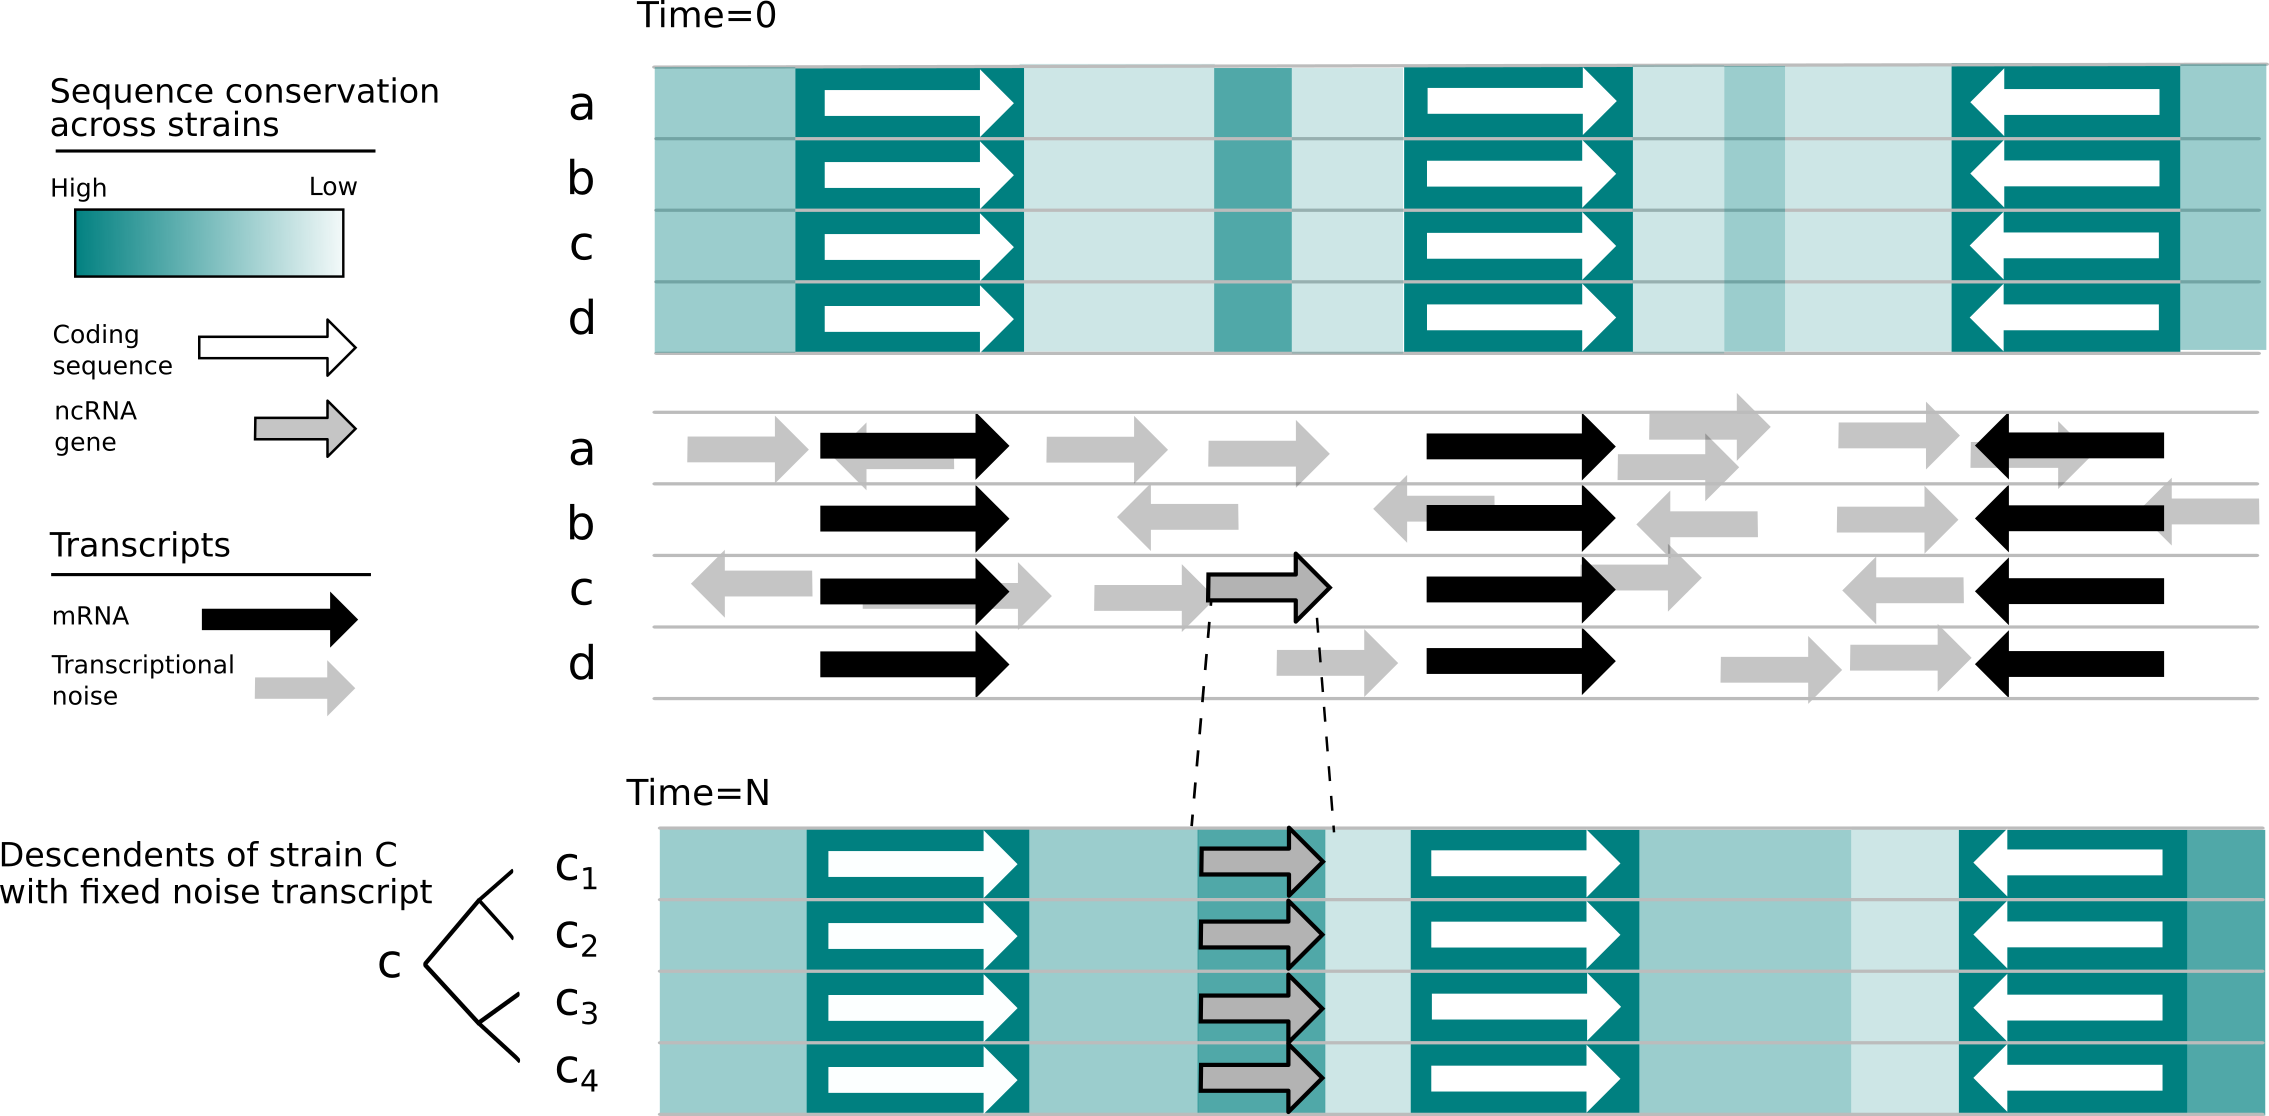
\includegraphics[scale=0.5]{lit_review/transcriptional_noise.png}
  \caption{Fixation of transcriptional noise. At Time=0: The top panel shows hypothetical genome sequences for four related bacterial strains (a, b, c, d) with regions of varying conservation along the sequence. The middle panel shows transcripts produced by each strain - dark colours indicate coding sequences, light colours indicate non-coding sequences. Noise transcripts are common, but not consistently expressed across strains and typically have low expression levels. At Time=N (bottom panel): In descendents of strain ‘C’ (C1, C2, C3, C4, C5) a noise transcript from the ancestral ‘C’ has been fixed due to drift, a selective sweep or population bottleneck.}
  \label{fig:transcriptional_noise}
\end{figure}

For the purposes of this review, we define transcriptional noise as transcription which does not have a fitness benefit to the organism in its native environment(s) sufficient to drive fixation, providing a null model for observed transcripts \citep{Koonin2016-wg}. While testing this condition in multicellular eukaryotic cells may prove difficult, the development of high-throughput approaches to phenotyping has made testing this condition theoretically tractable in most bacteria \citep{Gray2015-fv,Brochado2013-xy}, limited mainly by our understanding of and ability to model bacterial ecology. In particular, technologies like transposon insertion sequencing \citep{Chao2016-df}, CRISPRi \citep{Peters2015-qv}, and robotics platforms \citep{Kritikos2017-ym} are increasingly making it easier to test the fitness effects of genes in a range of physiologically relevant conditions. Applying these technologies in concert with experimental evolution (Cooper 2018) may allow for the calibration of the selection coefficients necessary to maintain a gene in a given population, at least under laboratory conditions.
 
\section{Estimating the rate of \textit{de novo} sRNA evolution}

So, how likely is the \textit{de novo} generation of a functional sRNA? We may never know for certain, but attempting to establish the parameters necessary to estimate this probability can help to clarify our expectations and direct investigation. In this back-of-the-envelope spirit, we have tried to lay out the key parameters for sRNA generation in Figure \ref{fig:drake}A, inspired by a similar Drake-like equation for the \textit{de novo} generation of protein-coding genes \citep{Weisman2017-gm}. This comprises three primary components: the transcript birth rate and the transcript death rate, which together establish the reservoir of transcriptional noise available for selection to act on,  and finally the probability of acquiring a beneficial function. The fitness effects of any particular nascent transcript on the host organism will represent a draw from the distribution of potential effects (Figure \ref{fig:drake}B). \par

\begin{figure}[H]
  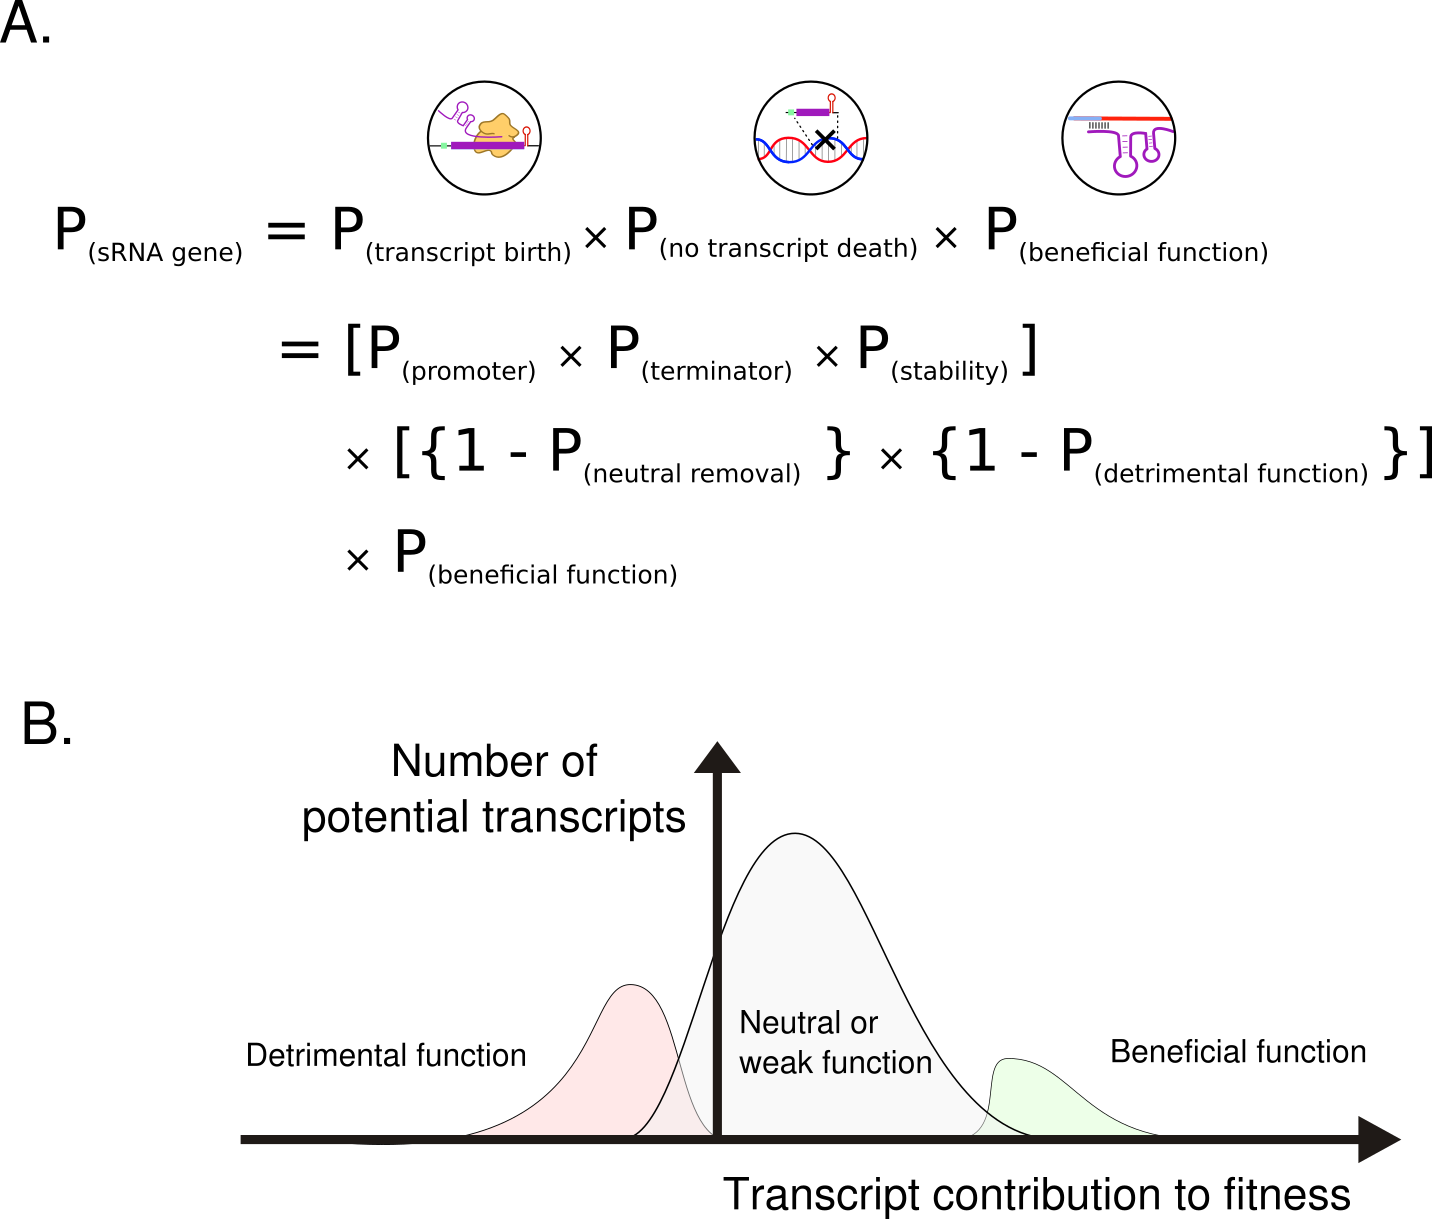
\includegraphics[scale=1.2]{lit_review/drake_eqn_final_2.png}
  \caption{(A) Estimating the probability of \textit{de novo} sRNA formation with a Drake-like equation. Details of each term are discussed in detail in the text. Briefly, the probability of sRNA formation has been decomposed into three relatively independent factors, the probabilities of transcript birth, transcript death and of acquiring a beneficial function. These probabilities can be further decomposed, into e.g. the probabilities of promoter and terminator acquisition, as well as acquiring stabilisation factors for the transcript birth probability.
(B) Theoretical distribution of fitness for potential transcripts of detrimental (red), neutral (grey) or beneficial (green) function. While P[beneficial function] and P[detrimental function] are not independent, they represent extremes of the distribution of potential transcript fitness, separated by a large number of transcripts with a neutral or "weak" function. (Based on Figure 1, \cite{Martin2016-re}) }
  \label{fig:drake}
\end{figure}

Transcript birth requires three basic components: promotion, termination, and transcript stabilization. A number of lines of evidence suggest the generation of spontaneous promoters is common. Many bacterial promoter sequences are degenerate, and transcription factor binding sites may arise from just a few point mutations \citep{Stone2001-yd}. This result has recently been confirmed by experimental evolution in \textit{E. coli} \citep{Yona2018-hx}, showing that random sequences can rapidly acquire promoter activity. These theoretical and laboratory results are supported by observations that antisense promoters are common \citep{Dornenburg2010-rq,Thomason2015-ky} but rarely conserved \citep{Raghavan2012-wr,Shao2014-hq}, suggesting a continuous turn-over in these sites.\par

It is less clear how transcriptional termination might evolve. Classical Rho-independent terminators are complex, requiring both a stable stem loop and poly-uridine stretch \citep{Ray-Soni2016-tw}. It is not obvious how they might frequently arise, though the frequent occurrence of inverted repeat structures in intergenic sequences suggests it may be possible \citep{Ladoukakis2008-zz,Lillo2002-wg}. These repeats, through their provision of secondary structure, might also serve as a reservoir of important stability determinants by protecting nascent transcripts from exonuclease digestion \citep{Dar2018-tq}.  The acquisition of secondary structures and/or associations with protective proteins may be especially important for the survival of non-coding transcripts, which unlike mRNAs do not benefit from protection against degradation by the presence of translating ribosomes \citep{Edri2014-av}. \par

Alternatives to \textit{de novo} evolution of Rho-independent terminators include the deposition of terminators by mobile elements \citep{Naville2010-jq}, or through genomic rearrangements, either of which could provide a space in which an sRNA could evolve. A recent study has indicated the generation of a genus-specific non-coding transcript through just such a rearrangement in \textit{Salmonella} \citep{Raghavan2015-wp}. Additionally, Rho-dependent termination appears to occur in a number of intergenic transcripts \citep{Peters2009-py}, although as the features promoting Rho recruitment are less well understood, the evolutionary implications of this are unclear.\par

Once expressed, a nascent transcript has to survive long enough to acquire function. Pervasive transcription from non-coding regions is now an accepted feature of eukaryotic genomes \citep{Deveson2017-vp}, and it appears selective constraints in eukaryotes are weak enough to allow for nearly every possible non-coding transcript to be sampled over evolutionary time \citep{Neme2016-ju}. However, relative to eukaryotes, bacteria have extremely compact genomes with gene contents averaging ~88\% \citep{Mira2001-mz}, reducing the sequence space available for the generation of intergenic transcriptional noise. This is driven by two factors: differences in mutational biases between bacteria and eukaryotes, and differences in the selective pressures felt by each.   \par

In contrast to eukaryotes, there is a strong bias towards deletion mutations in bacteria in the absence of selection \citep{Kudla2009-iw,Nilsson2005-lr}. This has important consequences for genome dynamics and the maintenance of non-coding sequence. In populations with small effective population sizes where selection is less effective, including many important human pathogens \citep{Weinert2017-pj}, genetic drift leads to reduced genome sizes \citep{Kuo2009-wd}. In these bacteria, transcript removal will be dominated by the neutral removal rate. Somewhat counterintuitively, this can also lead to a higher proportion of non-coding sequence in these genomes, due to the accumulation of pseudogenes and proliferation of selfish elements \citep{Novichkov2009-yy}.\par 

On the other hand, some environmental bacteria have large population sizes, increasing the effectiveness of selection in these populations compared to eukaryotes, and their smaller cell size increases their sensitivity to the energetic costs of gene maintenance relative to eukaryotes \citep{Lynch2015-lc}. Large population sizes may also make nascent transcripts more vulnerable to clonal interference \citep{Fogle2008-of}, where neutral or weakly beneficial mutations are rapidly removed through competition with other, more beneficial mutations that arise independently. As it is unlikely a novel transcript will be sufficient to confer a competitive advantage organism without time for selection to act, the rate of acquisition of beneficial mutation in the population as a whole will impact the rate of transcript fixation.\par  

Additional fitness costs may be imposed by the biochemical activity of the noise transcript itself, for instance through stochastic interactions with other transcripts \citep{Umu2016-he} — these may be increased by the relative lack of compartmentalization in bacterial cells. This selective pressure results in a reduced noncoding:coding DNA ratio \citep{Novichkov2009-yy}, in extreme cases leading to another form of genome reduction driven by streamlining \citep{Batut2014-hm} as observed in the SAR11 clade of marine bacteria \citep{Giovannoni2005-ab}.\par 

The final term in our Drake-like equation is acquisition of a beneficial function. Biochemical activity, in the form of affinity for other transcripts or RNA-binding proteins, would likely exist in any random transcript. However, such interactions are unlikely to have a strong effect on fitness prior to selection (Fig \ref{fig:drake}B). The observation that for many sRNAs, at least one of their target sites either pre-dates or originated at the same time as the sRNA \citep{Peer2014-yn} certainly suggests acquisition of interactions can be rapid; however, the majority of random interactions are likely detrimental to organismal fitness. As has been suggested for eukaryotic microRNAs \citep{Chen2007-mn}, bacterial noise transcripts that survive initial purification by selection are likely to have weak initial interactions with target genes, and low-level, condition-specific expression. Initial analysis of expression of young non-coding transcripts in \textit{Escherichia coli} and \textit{Salmonella enterica} suggest this is in fact the case \citep{Kacharia2017-fv}, and it has similarly been estimated that most antisense transcripts are expressed at levels too low to have major impacts on fitness \citep{Llorens-Rico2016-hv}. This line of argument also suggests affinity for RNA-binding proteins should follow a similar pattern. The ability to increase the effectiveness of interactions through acquisition of protein chaperone affinity (see box 1: RNA-binding proteins) may provide a route to rapidly tune the activity of a nascent sRNA.\par 

The terms in our sRNA Drake-like equation are of course all contingent on the specifics of each bacterial genome. Some examples include that genome-wide A/T content may make promoters and terminators more or less likely to occur \citep{Llorens-Rico2016-hv}, or that large effective population sizes may make selection more effective in some bacteria than others \citep{Novichkov2009-yy}, or that the presence of RNA-binding proteins may make sRNA-based regulation more effective in some lineages than others \citep{Peer2014-yn}. These terms can also be locally manipulated, by taking advantage of existing genomic features through the process of exaptation.\par

\subsection{Box 1: RNA-binding proteins}
Many sRNAs require RNA-binding proteins, such as Hfq, CsrA, and ProQ, to function \citep{Holmqvist2010-lc}. For instance, association with Hfq can greatly increase the rate of formation and the stability of sRNA-mRNA duplexes \citep{Fender2010-co,Panja2015-he}, and is necessary for the function of many \textit{E. coli} and \textit{Salmonella} trans-acting sRNAs. The requirement for Hfq appears to vary by genome, GC content, and sRNA composition, although studies are limited to a small number of model organisms with functionally characterised sRNAs \citep{Jousselin2009-tv}. Other sRNAs, such as the Csr/Rsm family, appear to operate primarily through titration of RNA-binding proteins themselves \citep{Romeo2018-wb}.\par

RNA-binding protein interaction sites appear to be relatively simple. Hfq has multiple binding surfaces with different sequence specificities \citep{Santiago-Frangos2018-xw}, primarily consisting of A- or U-rich tracts. The CsrA binding site is similarly small, requiring just a GGA sequence within a hairpin loop \citep{Romeo2018-wb}, though other factors can influence binding affinity \citep{Duss2014-lf}. The size and degeneracy of these motifs may provide a quick route to acquiring chaperone affinity, and many may require only small modifications of existing structures. For example, mutagenesis and CLIP-seq studies have shown that many Rho-independent terminators associate with Hfq \citep{Otaka2011-yc,Holmqvist2016-hj}. 

\section{Exaptation in the evolution of sRNAs}

Exaptation is the process through which existing features, sometimes referred to as pre-adaptations, are co-opted to provide a new function not previously selected for \citep{Gould1982-xk}. In the simplest case, processes such as duplication or horizontal transfer allow for transplantation of transcribed sequences, removing the need for \textit{de novo} evolution of promoters, terminators, or stability determinants and hence increasing the probability of sRNA generation. Importantly, both duplications and horizontal insertions provide non-deleterious sequences that are already adapted to the host, presenting a low-risk route to acquiring new ncRNAs. \par

Recognizable sRNA duplications appear fairly commonly \citep{Caswell2014-pk}. Notable examples including the Qrr sRNAs involved in quorum sensing in \textit{Vibrio} species \citep{Papenfort2016-mc}, the PrrF sRNAs involved in regulating iron homeostasis in \textit{Pseudomonas} \citep{Wilderman2004-le}, and the OmrA/B sRNAs in \textit{Escherichia coli} \citep{Holmqvist2010-lc}. Such duplications could allow duplicated sRNAs to diverge and gain new functions through a process of subfunctionalization and neofunctionalization \citep{Rastogi2005-hn}. While the functional divergence of duplicated sRNAs remains understudied, there are some tantalizing indications of regulon drift between duplicated sRNAs \citep{Caswell2014-pk}.\par 

Many bacterial genomes contain horizontally-acquired genomic islands (GIs) \citep{Dobrindt2004-as}, often referred to as pathogenicity islands in virulent bacteria, which are frequent sources of novel sRNAs \citep{Pichon2005-de,Padalon-Brauch2008-gh,Tree2014-wj}. The existence of such sRNAs is perhaps unsurprising, as many common mobile elements utilize ncRNA regulation to control their replication and integration \citep{Wagner1994-oj}, or to ensure their maintenance, such as the sRNA antitoxins in Type I toxin-antitoxin systems \citep{Brantl2012-ad}. One recent example of an apparent exaptation event is the \textit{art200} antisense RNA derived from \textit{tnpA} transposase loci that has been suggested to regulate \textit{Salmonella} Typhimurium virulence by targeting invasion genes \citep{Ellis2017-uv}, and may affect gastrointestinal colonization of mice \citep{Ellis2018-kf}. \par

\section{Protected spaces for sRNA evolution}

Beyond the direct duplication or import of transcriptional units, reusing the existing genome architecture provides another way to tweak the parameters of our Drake-like equation so as to increase the rate of sRNA formation. In particular, mRNA operon structures harbor expressed untranslated regions (UTRs) that are protected from large-scale deletions by the selective pressures maintaining the associated coding sequences, eliminating the need for \textit{de novo} evolution of transcription and lowering the probability of transcript removal. Recent work has suggested ncRNAs may be generated from within coding sequences themselves \citep{Dar2018-jq}, though no specific function has been proposed for these fragments as of yet.\par

3\textprime UTRs at the end of mRNA transcripts appear to be a particularly fertile ground for sRNA formation, with several instances well characterized \citep{Miyakoshi2015-gm}. The presence of rho-independent terminators at many gene ends provides a natural termination point, stable secondary structure, and possibly a precursor to an Hfq binding site (Box 1). The natural degradation of mRNA transcripts may by chance liberate such a stable fragment which is then free to acquire a secondary function. Indeed, such a stepwise evolution has been proposed for the CpxQ 3\textprime UTR derived sRNA \citep{Chao2016-df} (Figure \ref{fig:pathways_to_sRNA_evo}A). The expression of such sRNAs would be tied to the expression of their parent transcript, possibly limiting the functional space the sRNA could explore. A natural extension then would be the evolution of independent cryptic promoters that could unlink expression of the sRNA from the parent transcript. This is the case for the sRNA MicL expressed from the 3\textprime UTR of the cutC locus (Figure \ref{fig:pathways_to_sRNA_evo}B), which has been shown to be responsible for the copper sensitivity phenotype previously attributed to the coding sequence \citep{Guo2014-lq}. Intriguingly, MicL is transcribed as a 308 nucleotide sequence that is then processed to its active 80 nucleotide length. In fact, many well characterized intergenic sRNAs, for instance ArcZ \citep{Papenfort2009-tl}, are similarly processed. Are these processing sites genomic relics of a past 3\textprime UTR origin?\par

Many 5\textprime UTRs contain transcriptional attenuators, including riboswitches, RNA thermometers, peptide leaders, and RNA-binding protein motifs \citep{Naville2010-jq}. As a side-effect of attenuation some of these generate stable, or at least abundant, short transcripts that are then free to explore new functional spaces (Figure \ref{fig:pathways_to_sRNA_evo}C), though this would be constrained by the need to conserve the original attenuator function. Functionally characterised examples of such dual-purpose cis/trans regulators have been found derived from attenuators involved in virulence, such as the riboswitch-derived SreA in \textit{Listeria monocytogenes} \citep{Loh2009-is}, and the ATP- and charged tRNA-sensitive leader sequence of the \textit{Salmonella} mgtCBR operon \citep{Choi2017-zn}.\par

Beyond coding sequences, core ncRNAs such as ribosomal and tRNAs are often arranged in operons that are processed to generate functional molecules, producing various intermediates and byproducts along the way. The tRNAs have been proposed as promising candidates in particular \citep{Gottesman2011-cq}, as a number of tRNAs and their intermediates have been suggested to interact with Hfq \citep{Lee2008-ti,Zhang2003-pm}. Spacers excised from pre-tRNA transcripts during tRNA processing have been indeed found to act as sRNA sponges (Figure \ref{fig:pathways_to_sRNA_evo}D) \citep{Lalaouna2015-al}. Given the consistency of the tRNA complement across related species \citep{Marck2002-bm} it is unclear how often such transcripts might make the transition to independent sRNAs through duplication or decay of tRNA function, though the presence of enigmatic expressed repeats in the vicinity of some tRNA loci \citep{Bosl1991-nm} suggests it may be possible. A recent report has additionally suggested a role for Hfq in ribosomal RNA biogenesis \citep{Andrade2018-fs}, in particular providing evidence for Hfq binding of spacer regions flanking the mature 16S sequence, again raising the question of whether these sequences could acquire secondary functions.\par 


\begin{figure}[H]
  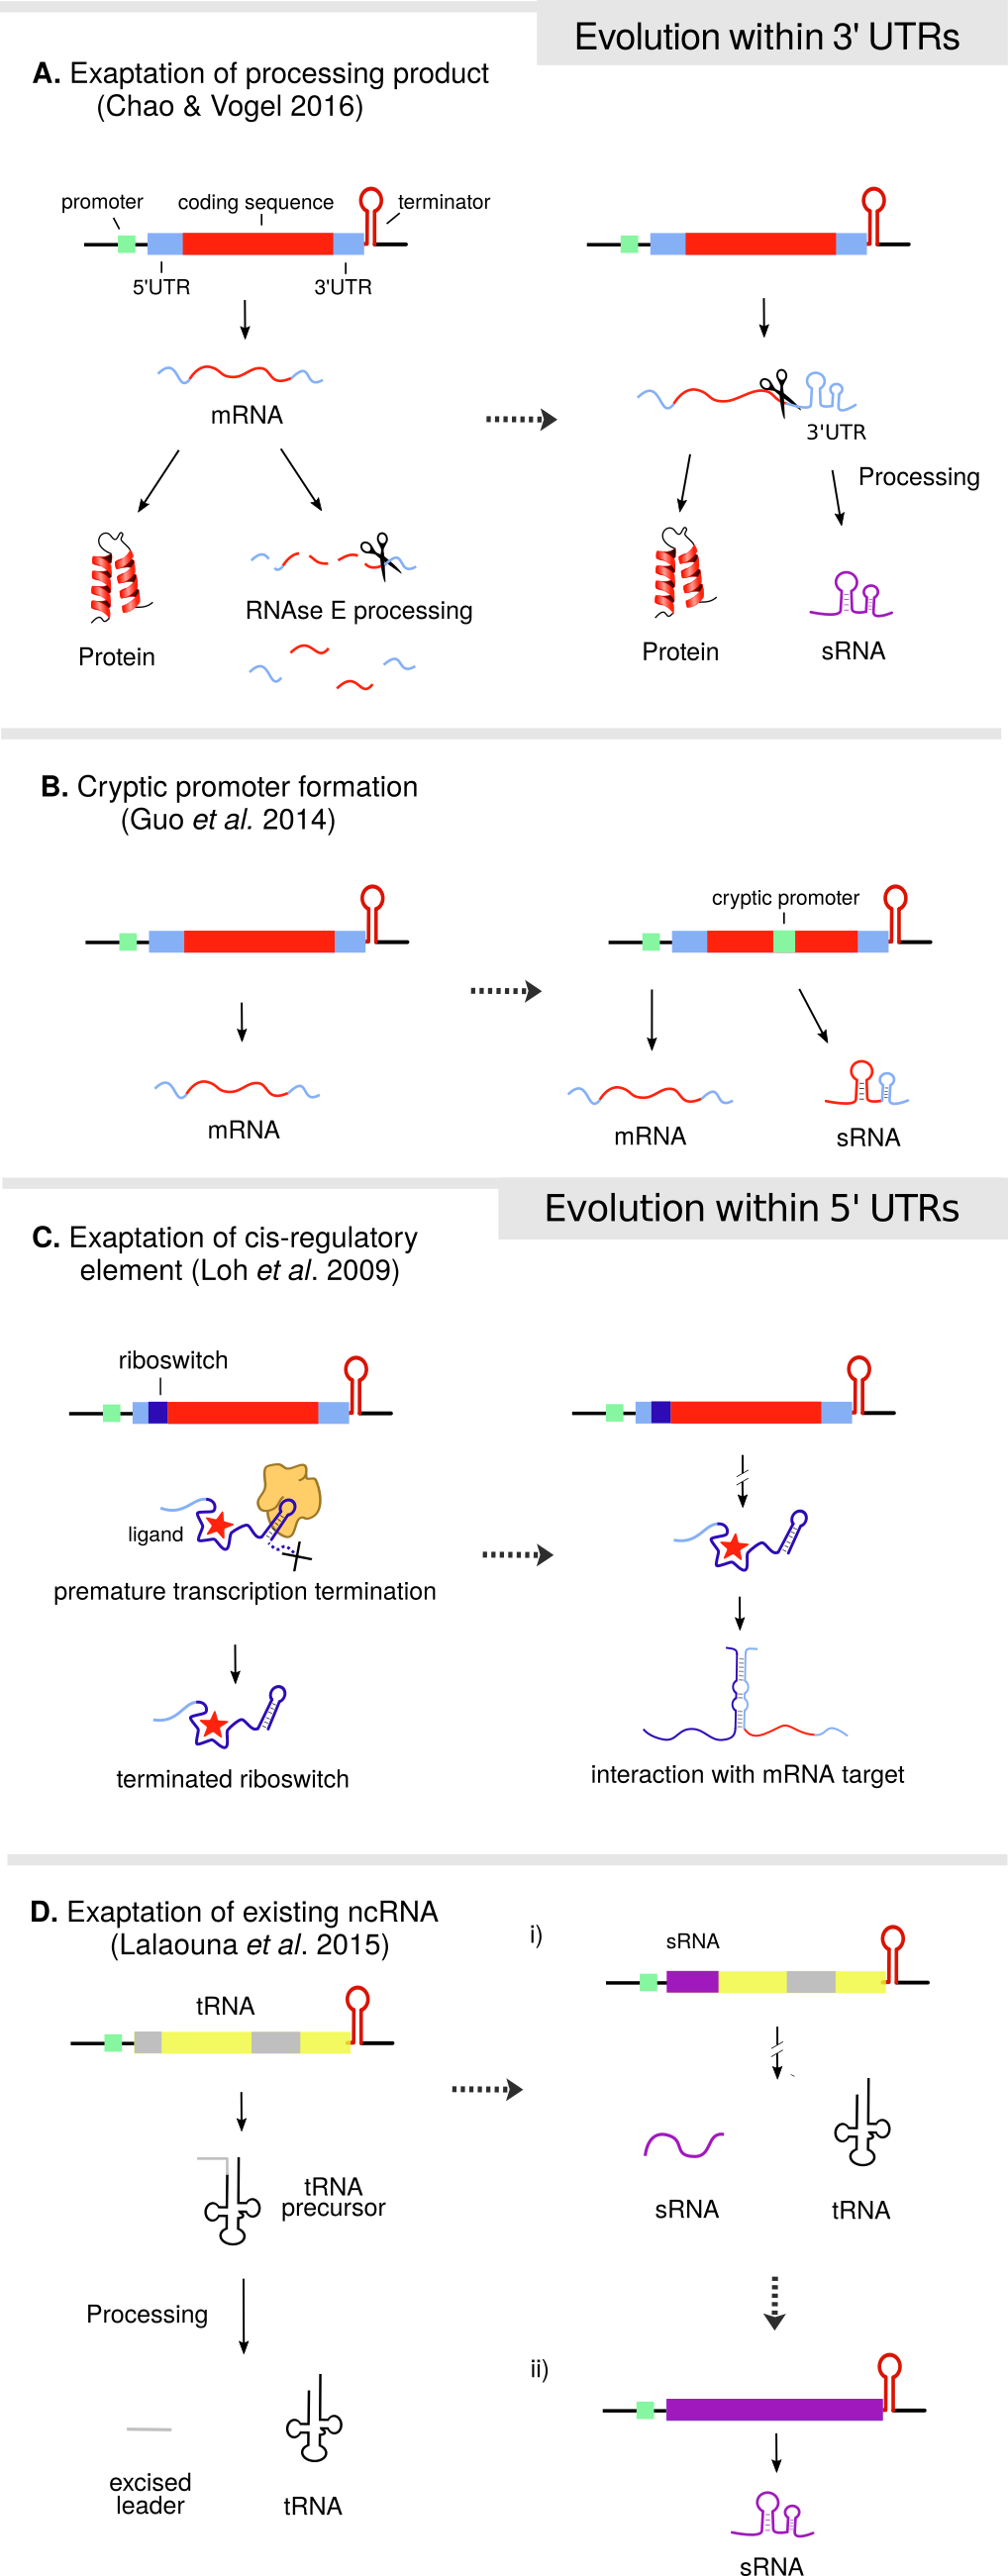
\includegraphics[scale=1]{lit_review/pathways_to_sRNA_evo_final_2.png}
  \caption{Routes for sRNA evolution within “protected spaces” - Functional genomic elements sheltered from deletion by selection on neighbouring genes, that may increase the probability of sRNA evolution. These include known examples from within 3\textprime UTRs, either derived from processing products (A), or cryptic promoters (B); from existing cis-regulatory elements in 5\textprime UTRs (C); or from existing ncRNAs, such as tRNAs (D).}
  \label{fig:pathways_to_sRNA_evo}
\end{figure}


\section{Future Directions} 

Here we have attempted to sketch the outline of a quantitative understanding of sRNA birth. Understanding the parameters of this equation will take significant work. One promising approach is through molecular archeology, attempting to infer the sequence of events that have lead to the present sRNA repertoire through the examination of increasingly plentiful bacterial genome sequences. Already, this approach has provided the first putative examples of sRNA creation through recombination \citep{Raghavan2015-wp}. Scaling this approach to the entire sRNA complement of a bacterial clade will be a challenge, with complications we have not touched upon in this review — for instance, the selective pressures we have examined are not constant but change as a bacterial population is exposed to different environmental circumstances. As many bacterial sRNAs appear to be involved in stress responses, these variable selective pressures may be particularly important to consider. Perhaps by combining this molecular archeology approach with new techniques for high-throughput characterization of sRNA function \citep{Barquist2015-ta}, we can begin to understand how transcriptional noise is domesticated to provide regulatory functions in the bacterial cell.\par

A second approach is to look forward, rather than back. Can we manipulate the terms of the sRNA formation equation to make it more likely that we observe the emergence of a functional bacterial sRNA under laboratory conditions? Could engineering the protected spaces we have reviewed here, coupled with the application of experimental evolution \citep{Cooper2018-oz,Cvijovic2018-lv}, provide a means for us to directly and reproducibly drive the \textit{de novo} birth of a gene? It is unclear how feasible this might be, but then aspirations do not need to be attainable to be useful.\par


\section{Acknowledgements}

The authors would like to thank Alex Westermann and Erik Holmqvist, and the anonymous reviewers for insightful comments on the draft manuscript.
\bibliographystyle{otago}
\bibliography{lit_review}


